% ======================================================================
% EXPERIMENTACIÓN Y RESULTADOS
% ======================================================================
\section{Experimentación y Resultados}
\label{ch:experimentacion}

Esta sección evalúa la extensión propuesta mediante experimentos diseñados para responder tres preguntas. ¿La codificación binaria y la codificación factorizada generan la misma función de valor óptima \(V^*\) y la misma política óptima \(\pi^*\) para un mismo MDP? ¿Reduce la codificación factorizada la complejidad del programa ProbLog que el modelador debe escribir respecto a la codificación binaria? ¿Cómo afecta la elección entre fluentes multivaluados o booleanos los tiempos de construcción del MDP y de resolución por Iteración de Valor?

% ------------------------------------------------------------------
\subsection{Diseño experimental}
\label{sec:exp-diseno}

\subsubsection{Dominios de evaluación}
\label{sec:exp-dominios}

El dominio primario es la familia de \textit{grids} de Mitchell
\cite{mitchell1997machine}, presentada en la Sección~\ref{sec:antecedentes}.
Sus transiciones deterministas permiten aislar el efecto de la codificación
sobre el tamaño del programa y el espacio de estados. Se evalúan ocho tamaños,
de $2\times3$ a $32\times32$ (Tabla~\ref{tab:exp-rq2}); el $2\times3$ sirve
como punto de verificación contra la solución publicada.

El dominio secundario es el \textit{grid} canónico $3\times4$ de Russell y
Norvig \cite{russell2016artificial}: $11$ estados, transiciones estocásticas
($0.80/0.10/0.10$), estado trampa en $(2,4)$ con recompensa $-1$ y costo por
paso de $-0.04$. Complementa al dominio Mitchell al verificar la corrección
de la extensión bajo distribuciones probabilísticas no triviales. Se evalúa en
una única instancia contra la Figura~17.3 de \cite{russell2016artificial}.

\subsubsection{Variables independientes}
\label{sec:exp-variables}

El experimento manipula dos variables independientes. La primera es la
\textbf{codificación del espacio de estados}: binaria o factorizada. La
codificación binaria se aplica únicamente al dominio Mitchell; la
factorizada se aplica a ambos dominios.

La segunda variable es la \textbf{configuración de inferencia}. ProbLog
dispone de dos \textit{backends} de compilación: circuitos d-DNNF
\cite{darwiche2003differential} y Diagramas de Decisión Sentencial (SDD)
\cite{darwiche2011sdd}. Para los circuitos d-DNNF se comparan dos evaluadores:
el estándar, que recorre el circuito una vez por consulta, y el diferencial de
Darwiche \cite{darwiche2003differential}, que calcula todas las marginales en
un único recorrido por diferenciación. El SDD usa el evaluador estándar de
ProbLog. A lo largo del capítulo, las tres configuraciones se identifican como
\textit{ddnnf}, \textit{darwiche} y \textit{sdd}, respectivamente.

\subsubsection{Protocolo de medición}
\label{sec:exp-protocolo}

El experimento comprende $50$ configuraciones: $48$ del dominio Mitchell
($8$ tamaños $\times$ $2$ codificaciones $\times$ $3$ configuraciones de
inferencia) y $2$ del dominio Russell (codificación factorizada con
\textit{ddnnf} y darwiche). El pipeline completo se ejecuta en cada corrida
desde cero: \textit{parsing}, clasificación de fluentes, \textit{grounding},
compilación del circuito e Iteración de Valor. Cada configuración se repite
$N = 10$ veces de forma independiente.

\clearpage

El límite de tiempo es de $400\,\text{s}$ por ejecución. Si una ejecución
supera ese límite, se registra con estado \texttt{TIMEOUT} y los datos
parciales disponibles. Los parámetros del solver se fijan en $\gamma = 0.9$
para el dominio Mitchell y $\gamma = 1.0$ para el dominio Russell, con
$\varepsilon = 0.01$ y $\varepsilon_{\text{thr}} = 10^{-6}$. Los tiempos
se miden con \texttt{time.perf\_counter()} dentro de cada corrida.

% ------------------------------------------------------------------
\subsection{Entorno de evaluación}
\label{sec:exp-entorno}

Los experimentos se ejecutaron sobre un equipo Intel\textregistered{} Core\texttrademark{} Ultra~7 155U (14 núcleos) con 16\,GB de RAM y sistema operativo Linux~6.17.0-20-generic. El intérprete fue Python~3.12.3. Las mediciones se realizaron en ejecuciones seriales; el proceso disponía de todos los recursos del equipo en cada corrida.

De las $50$ configuraciones, $43$ completaron las $10$ corridas dentro del límite de \textit{timeout}; las $7$ restantes registraron \texttt{TIMEOUT} en todas sus ejecuciones (Tabla~\ref{tab:exp-tiempos}).

% ------------------------------------------------------------------
\subsection{Corrección funcional}
\label{sec:exp-rq1}

Esta sección verifica que la extensión multivaluada produce la misma $V^*$
y la misma $\pi^*$ que la codificación binaria para un mismo MDP, y que
los resultados coinciden con la solución de referencia publicada.

\subsubsection{Verificación en el dominio Mitchell}
\label{sec:exp-rq1-mitchell}

La Tabla~\ref{tab:exp-correccion} compara $V^*(s)$ y $\pi^*(s)$ para cada
tamaño donde ambas codificaciones completaron. La columna $\max|\Delta V^*|$
reporta la diferencia máxima absoluta entre funciones de valor; la columna
Iter.\ el número de iteraciones de Bellman hasta convergencia. La tolerancia
de comparación es $10^{-6}$.

\begin{table}[htbp]
    \centering
    \caption{Verificación cruzada de corrección funcional en el dominio Mitchell.}
    \label{tab:exp-correccion}
    \small
    \begin{tabular}{l r r c c r}
        \toprule
        \textbf{Grid} & $|\mathcal{S}|_{\text{bin}}$ & $|\mathcal{S}|_{\text{fac}}$ & $\max|\Delta V^*|$ & \textbf{$\pi^*$ coincide} & \textbf{Iter.} \\
        \midrule
        $2 \times 3$   &    8 &    6 & 0.0 & Sí & 3  \\
        $3 \times 3$   &   16 &    9 & 0.0 & Sí & 3  \\
        $4 \times 4$   &   32 &   16 & 0.0 & Sí & 4  \\
        $6 \times 6$   &   64 &   36 & 0.0 & Sí & 6  \\
        $8 \times 8$   &  128 &   64 & 0.0 & Sí & 8  \\
        $12 \times 12$ &  256 &  144 & 0.0 & Sí & 12 \\
        $16 \times 16$ &  512 &  256 & 0.0 & Sí & 16 \\
        \bottomrule
    \end{tabular}
    \smallskip\\
    \footnotesize{El \textit{grid} $32 \times 32$ no aparece porque la codificación binaria superó el \textit{timeout} en las tres configuraciones de inferencia; la verificación cruzada requiere que ambas codificaciones completen.}
\end{table}

Las diferencias son exactamente $0.0$ en todos los tamaños evaluados y las
políticas coinciden en cada caso. Ambas codificaciones representan el mismo
MDP; la estructura de transiciones y recompensas es idéntica, por lo que la
Iteración de Valor converge en el mismo número de pasos con los mismos
parámetros $\gamma$ y $\varepsilon$ \cite{puterman2014markov}. La
verificación del dominio Russell se presenta en la
Sección~\ref{sec:exp-russell}.

% TODO [FIGURA]: Visualización de la política óptima π* sobre el grid 2×3 original de Mitchell.
%   Tipo: Grid 2×3 con flechas de acción en cada celda no terminal.
%   Contenido: 6 celdas, terminal en esquina superior derecha marcada con recompensa +100.
%     Flecha por celda mostrando la acción óptima. Coincide con Mitchell (1997).
%   Label sugerido: fig:politica-mitchell-2x3

% ------------------------------------------------------------------
\subsection{Simplificación del modelado}
\label{sec:exp-rq2}

Esta sección evalúa la reducción de complejidad en el
programa ProbLog. La Tabla~\ref{tab:exp-rq2} compara, para ambas
codificaciones y los ocho tamaños de \textit{grid}, el número de fluentes,
las cardinalidades de sus dominios, el número de reglas, el tamaño del espacio
de estados $|\mathcal{S}|$ y los estados espurios. Para la codificación
binaria, la columna Cardinalidades indica el número de bits; para la
factorizada, las cardinalidades de los dos fluentes multivaluados.

\begin{table}[htbp]
    \centering
    \caption{Métricas del programa fuente por codificación y tamaño de \textit{grid}.}
    \label{tab:exp-rq2}
    \small
    \begin{tabular}{l l r c r r r}
        \toprule
        \textbf{Grid} & \textbf{Cod.} & \textbf{Fluentes} & \textbf{Cardinalidades} & \textbf{Reglas} & $|\mathcal{S}|$ & \textbf{Esp.} \\
        \midrule
        \multirow{2}{*}{$2 \times 3$}
            & Bin. & 3 & $3$ bits        &    42 &    8 &   2 \\
            & Fac. & 2 & $2 \times 3$    &    21 &    6 &   0 \\
        \addlinespace
        \multirow{2}{*}{$3 \times 3$}
            & Bin. & 4 & $4$ bits        &    77 &   16 &   7 \\
            & Fac. & 2 & $3 \times 3$    &    21 &    9 &   0 \\
        \addlinespace
        \multirow{2}{*}{$4 \times 4$}
            & Bin. & 5 & $5$ bits        &   178 &   32 &  16 \\
            & Fac. & 2 & $4 \times 4$    &    21 &   16 &   0 \\
        \addlinespace
        \multirow{2}{*}{$6 \times 6$}
            & Bin. & 6 & $6$ bits        &   472 &   64 &  28 \\
            & Fac. & 2 & $6 \times 6$    &    21 &   36 &   0 \\
        \addlinespace
        \multirow{2}{*}{$8 \times 8$}
            & Bin. & 7 & $7$ bits        & 1\,025 &  128 &  64 \\
            & Fac. & 2 & $8 \times 8$    &    21 &   64 &   0 \\
        \addlinespace
        \multirow{2}{*}{$12 \times 12$}
            & Bin. & 8 & $8$ bits        & 2\,595 &  256 & 112 \\
            & Fac. & 2 & $12 \times 12$  &    21 &  144 &   0 \\
        \addlinespace
        \multirow{2}{*}{$16 \times 16$}
            & Bin. & 9 & $9$ bits        & 5\,376 &  512 & 256 \\
            & Fac. & 2 & $16 \times 16$  &    21 &  256 &   0 \\
        \addlinespace
        \multirow{2}{*}{$32 \times 32$}
            & Bin. & 11 & $11$ bits     & $26\,623$ & $2\,048$ & $1\,024$ \\
            & Fac.  &  2 & $32 \times 32$ &    21 & $1\,024$ &   0 \\
        \bottomrule
    \end{tabular}
    \smallskip\\

\end{table}

La codificación factorizada mantiene $21$ reglas para cualquier tamaño de
\textit{grid}; la binaria escala de $42$ a $26\,623$ en el mismo rango. La
codificación factorizada no genera estados espurios; la binaria los acumula
con cada incremento de escala. La Figura~\ref{fig:reglas-celdas} ilustra
esta divergencia.

El \textit{grid} $4\times4$ presenta una restricción adicional. Sus $16$
celdas requieren $4$ bits como mínimo, pero la implementación no puede usar
el estado~$0$ para modelar transiciones, lo que fuerza el uso de $5$ bits y
genera $16$ estados espurios. Esta restricción afecta cualquier \textit{grid}
cuyo número de celdas sea una potencia exacta de~$2$.

\begin{figure}[htbp]
    \centering
    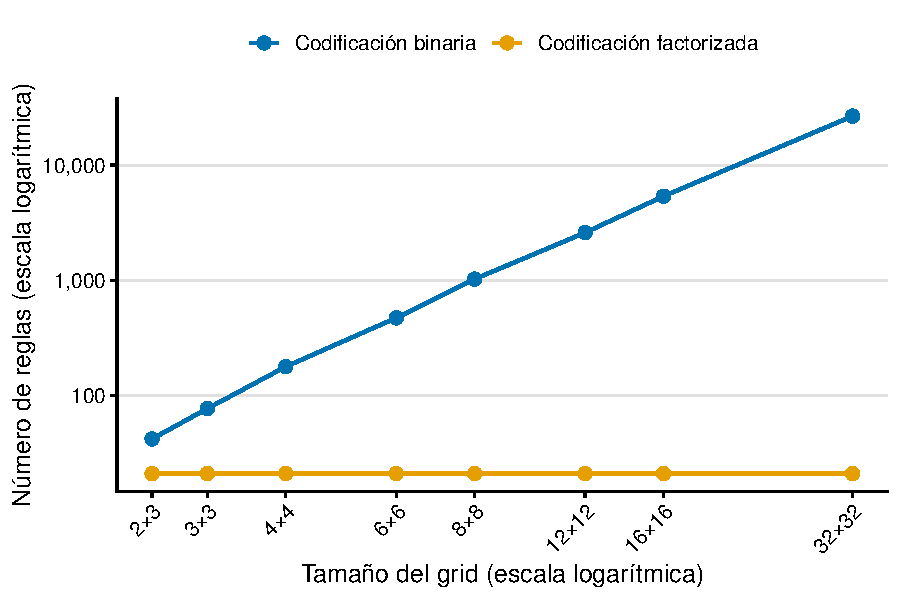
\includegraphics[width=0.85\textwidth]{figuras/reglas-celdas.pdf}
    \caption{Número de reglas del programa fuente en función del número de celdas del \textit{grid}.}
    \label{fig:reglas-celdas}
\end{figure}

\clearpage

% ------------------------------------------------------------------
\subsection{Impacto computacional}
\label{sec:exp-rq3}

Esta sección evalúa cómo influye la elección de codificación sobre el rendimiento del solver. La fase de construcción ($t_{\text{build}}$) abarca \textit{parsing}, clasificación de fluentes, \textit{grounding} y compilación del circuito. La fase de Iteración de Valor ($t_{\text{VI}}$) ejecuta las actualizaciones de Bellman hasta convergencia. El tiempo total es $t_{\text{total}} = t_{\text{build}} + t_{\text{VI}}$.

\subsubsection{Tiempos de ejecución}
\label{sec:exp-tiempos}

La Tabla~\ref{tab:exp-tiempos} presenta $t_{\text{total}}$ para cada combinación de codificación y configuración de inferencia. Las configuraciones que completaron reportan media y desviación estándar sobre $10$ ejecuciones independientes.

\begin{table}[htbp]
    \centering
    \caption{Tiempo total de ejecución $t_{\text{total}}$ (segundos) por codificación y configuración de inferencia.}
    \label{tab:exp-tiempos}
    \footnotesize
    \begin{tabular}{l l r r r}
        \toprule
        \textbf{Grid} & \textbf{Cod.} &
            \textbf{ddnnf} (s) &
            \textbf{darwiche} (s) &
            \textbf{sdd} (s) \\
        \midrule
        \multirow{2}{*}{$2 \times 3$}
            & Bin. & $0.218 \pm 0.117$ & $0.109 \pm 0.005$ & $0.056 \pm 0.003$ \\
            & Fac. & $0.237 \pm 0.014$ & $0.103 \pm 0.008$ & $0.059 \pm 0.018$ \\
        \addlinespace
        \multirow{2}{*}{$3 \times 3$}
            & Bin. & $0.805 \pm 0.037$ & $0.379 \pm 0.016$ & $0.100 \pm 0.001$ \\
            & Fac. & $0.504 \pm 0.015$ & $0.175 \pm 0.029$ & $0.067 \pm 0.005$ \\
        \addlinespace
        \multirow{2}{*}{$4 \times 4$}
            & Bin. & $4.37 \pm 0.05$   & $1.52 \pm 0.03$   & $0.315 \pm 0.036$ \\
            & Fac. & $1.14 \pm 0.02$   & $0.283 \pm 0.017$ & $0.100 \pm 0.003$ \\
        \addlinespace
        \multirow{2}{*}{$6 \times 6$}
            & Bin. & $27.8 \pm 2.6$    & $6.98 \pm 0.13$   & $1.11 \pm 0.04$   \\
            & Fac. & $4.22 \pm 0.14$   & $0.701 \pm 0.031$ & $0.244 \pm 0.028$ \\
        \addlinespace
        \multirow{2}{*}{$8 \times 8$}
            & Bin. & $131.8 \pm 6.4$   & $32.9 \pm 1.2$    & $4.20 \pm 0.57$   \\
            & Fac. & $10.8 \pm 0.6$    & $1.40 \pm 0.04$   & $0.507 \pm 0.033$ \\
        \addlinespace
        \multirow{2}{*}{$12 \times 12$}
            & Bin. & \texttt{TIMEOUT}.              & $161 \pm 3.4$     & $20.5 \pm 1.3$    \\
            & Fac. & $68.9 \pm 3.1$    & $5.36 \pm 0.12$   & $1.82 \pm 0.05$   \\
        \addlinespace
        \multirow{2}{*}{$16 \times 16$}
            & Bin. & \texttt{TIMEOUT}.              & \texttt{TIMEOUT}.              & $94.2 \pm 10.2$   \\
            & Fac. & $245 \pm 2.3$     & $14.8 \pm 0.6$    & $5.11 \pm 0.46$   \\
        \addlinespace
        \multirow{2}{*}{$32 \times 32$}
            & Bin. & \texttt{TIMEOUT}.              & \texttt{TIMEOUT}.              & \texttt{TIMEOUT}.              \\
            & Fac. & \texttt{TIMEOUT}.              & $189 \pm 10$      & $58.9 \pm 3.8$    \\
        \bottomrule
    \end{tabular}
\end{table}

Los tiempos de la codificación binaria crecen más rápido que los de la factorizada a medida que aumenta el tamaño del grid. La Iteración de Valor domina $t_{\text{total}}$ en la mayoría de las configuraciones. 

\clearpage

\subsubsection{Cociente de tiempos entre codificaciones}
\label{sec:exp-speedup}

La Tabla~\ref{tab:exp-speedup} presenta el cociente $t_{\text{total}}^{\text{bin}} / t_{\text{total}}^{\text{fac}}$ para los pares donde ambas codificaciones completaron. \texttt{TIMEOUT} indica que la codificación binaria superó el límite de tiempo mientras que la factorizada no. Un valor menor que $1.0$ indica que la binaria fue más rápida.

\begin{table}[htbp]
    \centering
    \caption{Cociente de tiempos $t_{\text{total}}^{\text{bin}} / t_{\text{total}}^{\text{fac}}$ por configuración de inferencia.}
    \label{tab:exp-speedup}
    \small
    \begin{tabular}{l r r r}
        \toprule
        \textbf{Grid} & \textbf{ddnnf} & \textbf{darwiche} & \textbf{sdd} \\
        \midrule
        $2 \times 3$   & $0.92\times$ & $1.06\times$ & $0.95\times$ \\
        $3 \times 3$   & $1.60\times$ & $2.17\times$ & $1.49\times$ \\
        $4 \times 4$   & $3.82\times$ & $5.36\times$ & $3.15\times$ \\
        $6 \times 6$   & $6.59\times$ & $9.96\times$ & $4.56\times$ \\
        $8 \times 8$   & $12.2\times$ & $23.6\times$ & $8.28\times$ \\
        $12 \times 12$ & \texttt{TIMEOUT}.   & $30.0\times$ & $11.2\times$ \\
        $16 \times 16$ & \texttt{TIMEOUT}.   & \texttt{TIMEOUT}.   & $18.4\times$ \\
        \bottomrule
    \end{tabular}
\end{table}

Para el \textit{grid} $2\times3$, las configuraciones \textit{ddnnf} y \textit{sdd} muestran cocientes menores a $1.0$. A partir de $3\times3$, la codificación factorizada supera a la binaria en las tres configuraciones de inferencia..

La inversión de rendimiento entre $2\times3$ y $3\times3$ refleja el costo fijo de las Disyunciones Anotadas. Para el tamaño mínimo, el \textit{overhead} de compilar los nodos \textit{choice} supera la ventaja de un espacio de estados reducido; a partir de $3\times3$, la reducción de estados y cláusulas lo compensa.

\subsubsection{Comparación de configuraciones de inferencia}
\label{sec:exp-backends}

Las tres configuraciones de inferencia difieren en su velocidad y en la tasa de crecimiento con el tamaño del \textit{grid}. El análisis se realiza sobre la codificación factorizada, que ofrece el mayor número de configuraciones completadas.

La configuración \textit{sdd} produce los tiempos más bajos en todos los tamaños evaluados. La configuración darwiche es entre $1.75\times$ y $3.2\times$ más lenta que \textit{sdd}. La configuración \textit{ddnnf} muestra la tasa de crecimiento más alta: en $4 \times 4$ es $4.0\times$ más lenta que darwiche, y en $16 \times 16$ esa diferencia es $16.5\times$.

La diferencia entre \textit{ddnnf} y \textit{darwiche} confirma el análisis de la Sección~\ref{sec:di-darwiche}. La ventaja de \textit{sdd} frente a d-DNNF excede el alcance de este trabajo. Los tiempos se reportan solo como observación empírica. La Figura~\ref{fig:tiempos-total} presenta las seis series.

\begin{figure}[htbp]
    \centering
    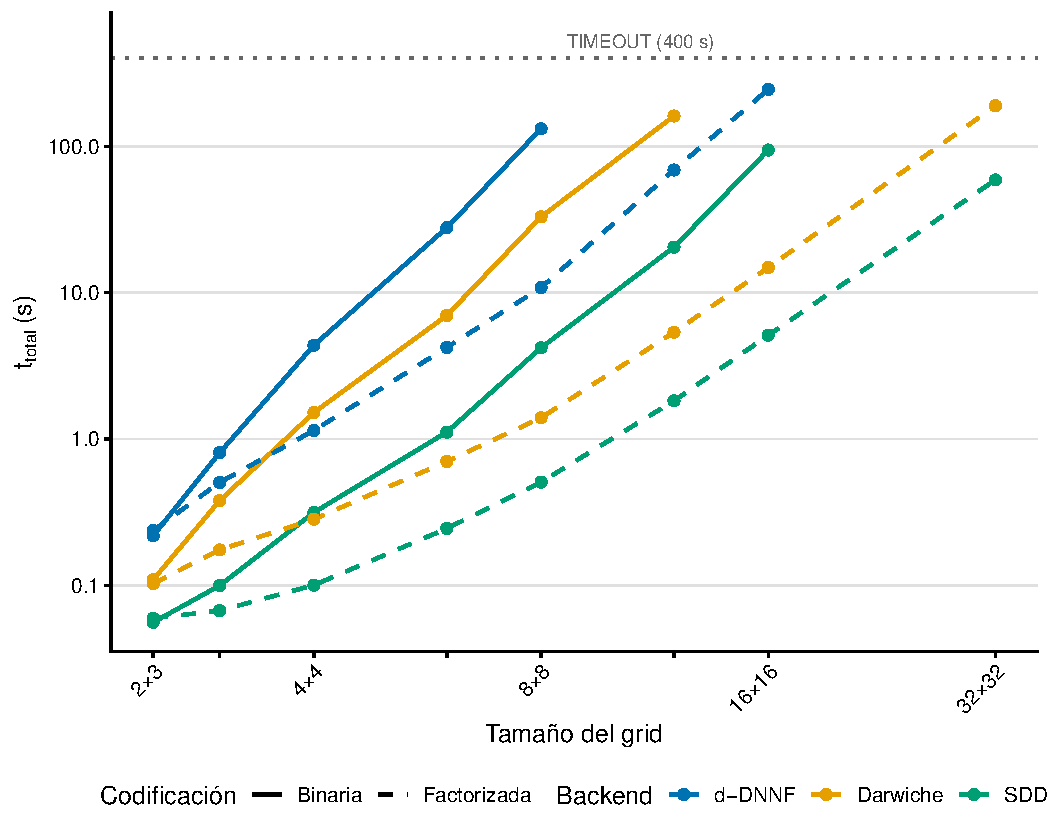
\includegraphics[width=0.92\textwidth]{figuras/tiempos-total.pdf}
    \caption{Tiempo total de ejecución en función del número de celdas del \textit{grid} para las seis combinaciones codificación~$\times$~\textit{backend}.}
    \label{fig:tiempos-total}
\end{figure}

\clearpage
% ------------------------------------------------------------------
\subsection{Dominio Russell}
\label{sec:exp-russell}

El dominio de Mitchell utiliza transiciones deterministas, lo que aísla el efecto de la representación pero no verifica la extensión bajo condiciones estocásticas. El dominio canónico $3 \times 4$ de Russell y Norvig \cite{russell2016artificial} complementa esta evaluación con transiciones probabilísticas, un estado trampa y un costo por paso. La evaluación se realiza con la codificación factorizada, que expresa la posición del agente como un fluente multivaluado \texttt{coor(X,Y)} con $11$ valores posibles y un programa fuente de $50$ reglas. Las configuraciones de inferencia evaluadas son \textit{ddnnf} y darwiche; la configuración \textit{sdd} produjo un error de compilación en este dominio y queda fuera del análisis cuantitativo.

\subsubsection{Verificación de la función de valor óptima}
\label{sec:exp-russell-v}

La función de valor óptima $V^*(s)$ se verificó contra la Figura~17.3 de Russell y Norvig \cite{russell2016artificial}, con los parámetros canónicos del dominio ($\gamma = 1.0$, $R = -0.04$). La columna $|\Delta V^*|$ reporta la diferencia absoluta entre el valor obtenido por el solver y el valor de referencia.

\begin{table}[htbp]
    \centering
    \caption{Verificación de $V^*(s)$ frente a la solución de referencia para el dominio Russell $3 \times 4$.}
    \label{tab:exp-russell-v}
    \small
    \begin{tabular}{c c r r}
        \toprule
        \textbf{Fila} & \textbf{Columna} & $V^*$ \textbf{(referencia)} & $|\Delta V^*|$ \\
        \midrule
        3 & 1 & 0.812 & $< 0.001$ \\
        3 & 2 & 0.868 & $< 0.001$ \\
        3 & 3 & 0.918 & $< 0.001$ \\
        2 & 1 & 0.762 & $< 0.001$ \\
        2 & 3 & 0.660 & $< 0.001$ \\
        1 & 1 & 0.705 & $< 0.001$ \\
        1 & 2 & 0.655 & $< 0.001$ \\
        1 & 3 & 0.611 & $< 0.001$ \\
        1 & 4 & 0.388 & $< 0.001$ \\
        \midrule
        3 & 4 & meta ($+1$)    & 0.000 \\
        2 & 4 & trampa ($-1$)  & 0.000 \\
        \bottomrule
    \end{tabular}
    \smallskip\\
    \footnotesize{Las coordenadas $(X, Y)$ siguen la convención del modelo: fila $X = 1$ en la base del \textit{grid}, columna $Y = 1$ a la izquierda. El estado $(2,2)$ es un obstáculo y no pertenece al espacio de estados.}
\end{table}

Los nueve estados no terminales presentan diferencias menores a $0.001$ respecto a los valores de referencia, y la política óptima $\pi^*$ obtenida coincide con la Figura~17.2 de Russell y Norvig \cite{russell2016artificial}. Los estados terminales tienen $V^* = 0$ en el solver, consistente con la semántica de absorción.

% TODO [FIGURA]: Visualización de la política óptima π* sobre el grid 3×4 de Russell.
%   Tipo: Grid con flechas de acción en cada celda no terminal.
%   Contenido: 12 celdas, obstáculo en (2,2), meta en (3,4), trampa en (2,4).
%   Flecha en cada celda no terminal y no obstáculo mostrando π*(s).
%   Label sugerido: fig:russell-policy

% ------------------------------------------------------------------

\clearpage

\subsection{Discusión}
\label{sec:exp-discusion}

La extensión preserva la semántica del MDP. Los resultados de las
Secciones~\ref{sec:exp-rq1} y~\ref{sec:exp-russell} confirman que la
codificación multivaluada produce la misma $V^*$ y la misma $\pi^*$ que
la codificación binaria tanto en condiciones deterministas como estocásticas.
Esta compatibilidad es consecuencia de que ambas codificaciones representan
el mismo MDP subyacente. La estructura de transiciones y recompensas es
idéntica, de modo que la Iteración de Valor converge en el mismo número de
pasos con los mismos parámetros \cite{puterman2014markov}.

Los datos de la Tabla~\ref{tab:exp-rq2} muestran que la codificación
factorizada reduce el tamaño del programa fuente de manera consistente en
todos los tamaños evaluados. El número de reglas se mantiene en $21$
independientemente de la escala del dominio, mientras que la codificación
binaria escala de $42$ reglas en el grid $2 \times 3$ hasta $26\,623$ en
el grid $32 \times 32$. Esta constancia es una consecuencia directa de que
la codificación multivaluada describe la dinámica en términos de los valores
naturales del dominio, sin necesidad de expandir cada variable en múltiples
predicados booleanos. La reducción del número de reglas va acompañada de
la eliminación de los estados espurios, lo que reduce el número de pares
$(s, a)$ que el \textit{solver} evalúa en cada iteración de Bellman.

La codificación multivaluada y el evaluador de Darwiche producen efectos
que se amplifican mutuamente. La codificación factorizada reduce $|\mathcal{S}|$
y, con ello, el número de pares $(s, a)$ por iteración. El evaluador de
Darwiche \cite{darwiche2003differential} elimina el factor $Q$ del costo de
cada par al calcular todas las marginales en dos pasadas lineales sobre el
circuito. Ambos efectos escalan con el tamaño del \textit{grid}, lo que
explica el crecimiento del cociente en la Tabla~\ref{tab:exp-speedup}. El
grid $2 \times 3$ constituye un caso límite donde la diferencia entre espacios
de estados ($8$ frente a $6$~estados) no compensa el costo fijo de compilar
los nodos \textit{choice} que implementan las Disyunciones Anotadas; a partir
del grid $3 \times 3$, la reducción del espacio de estados domina el
\textit{overhead} de compilación y la codificación factorizada supera a la
binaria en las tres configuraciones de inferencia evaluadas.

Los resultados son válidos dentro del alcance evaluado. Los dominios Mitchell
son \textit{grids} regulares sin obstáculos, con transiciones deterministas y
un único fluente; la generalización a dominios con múltiples fluentes
dependientes, transiciones complejas u obstáculos requiere evaluación
adicional. El dominio Russell aporta verificación estocástica en una única
instancia de $11$ estados, insuficiente para derivar tendencias de
escalamiento. El comportamiento de la configuración \textit{sdd} en dominios
estocásticos queda como cuestión abierta; el error de compilación observado
en el dominio Russell no fue diagnosticado en este trabajo.
